\documentclass[10pt,letterpaper]{article}
\usepackage[latin1]{inputenc}
\usepackage[light]{iwona}
\usepackage[T1]{fontenc}
\usepackage{newtxsf} % Make math pretty
\usepackage{cornell}
\usepackage{fancyhdr}
\usepackage{lastpage}
\usepackage{graphicx}
\usepackage{float}
\usepackage{titlesec}
\usepackage{siunitx}
\usepackage{parskip} 
\setlength{\parskip}{.1cm}
\usepackage{sagetex}

\cornelltitle{Trilateration Equation and Error}{Dawson Beatty}
\author{}

\pagestyle{fancy}
\fancyhf{}
\renewcommand{\sectionmark}[1]{\markright{#1}}
\lhead{\fancyplain{}{\rightmark }}
\rhead{}
\renewcommand{\footrulewidth}{1pt}
\renewcommand{\headrulewidth}{1.2pt}
\cfoot{Page \thepage\hspace{.03cm} of \pageref{LastPage}}
\lfoot{Project DRAGON}
\rfoot{University of Colorado at Boulder}


\titleformat{\section}
  {\normalfont\Large\bfseries}{\thesection}{1em}{}[{\titlerule[0.01cm]}]

\begin{document}
\maketitle

\setcounter{tocdepth}{4}
\tableofcontents

\newpage

% ===== Basic Trilateration =====
\section{Basic Trilateration}

Premise of trilateration is that there are three beacons from which the distance can be measured. Need at least three beacons for unique intersection.

\begin{figure}[H]
\centering
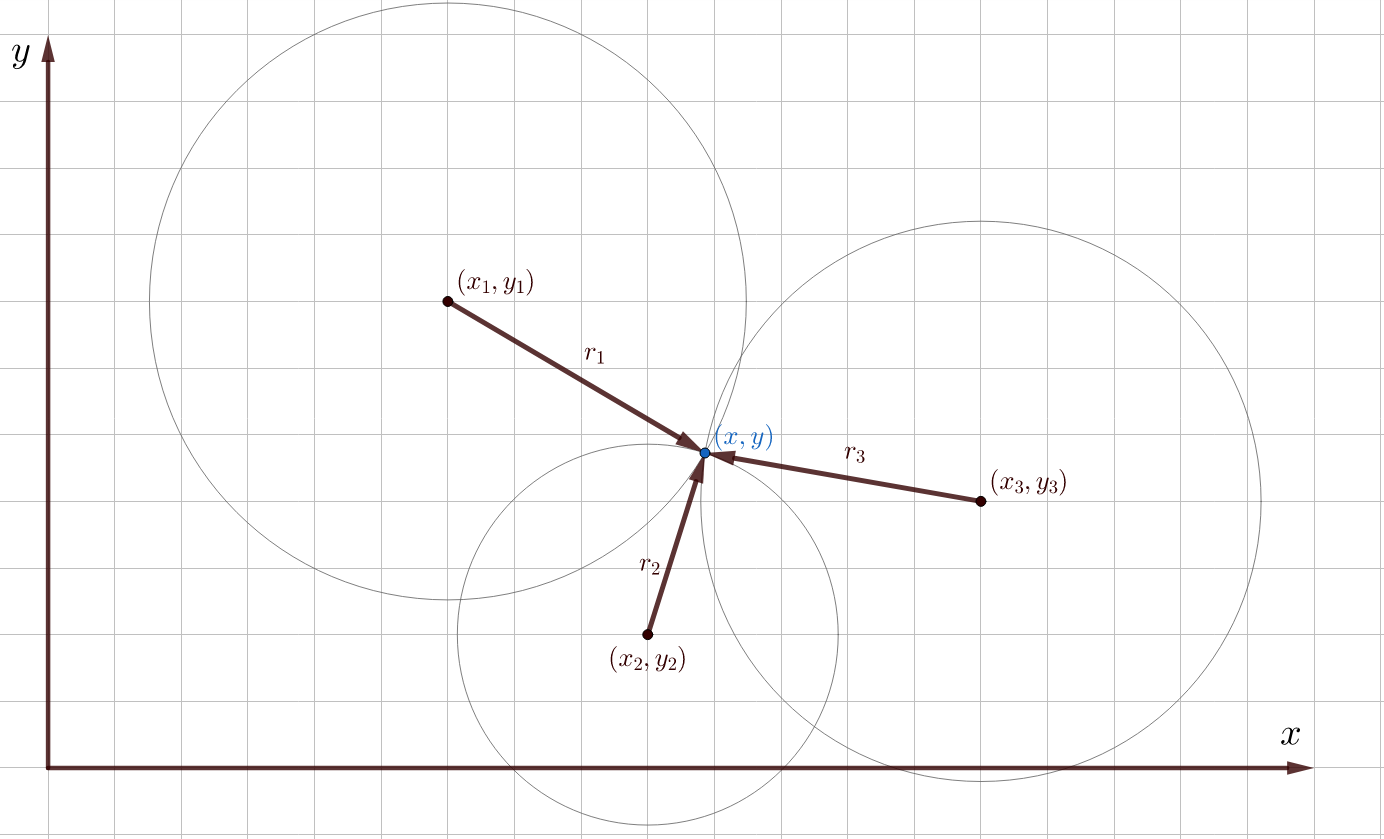
\includegraphics[width=.6\textwidth]{trilateration.png}
\end{figure}

\begin{sagesilent}
x, x_1, x_2, x_3, y, y_1, y_2, y_3 = var('x', 'x_1', 'x_2', 'x_3', 'y', 'y_1', 'y_2', 'y_3')

r_1, r_2, r_3 = var('r_1', 'r_2', 'r_3')
 
distance1 = ( -2 * x_1 + 2 * x_2) * x + (-2 * y_1 + 2 * y_2) * y == r_1 ** 2 - r_2 ** 2 - x_1 ** 2 + x_2 ** 2 - y_1 ** 2 + y_2 ** 2 
distance2 = ( -2 * x_2 + 2 * x_3) * x + (-2 * y_2 + 2 * y_3) * y == r_2 ** 2 - r_3 ** 2 - x_2 ** 2 + x_3 ** 2 - y_2 ** 2 + y_3 ** 2
 
res = solve([distance1, distance2], x, y)

x_func = res[0][0].right()
x = x_func
y_func = res[0][1].right()
y = y_func
\end{sagesilent}

Need to find point $(x, y)$ which satisfies all of these equations:

\begin{align*}
    (x - x_1) ^ 2 + (y - y_1) ^ 2 &= r_1^2 \\
    (x - x_2) ^ 2 + (y - y_2) ^ 2 &= r_2^2 \\
    (x - x_3) ^ 2 + (y - y_3) ^ 2 &= r_3^2 \\ 
\end{align*}

Subtract 2 from 1, 3 from 2. Forms system of equations which can be solved. 

\begin{align*}
    -2 \, x {\left(x_{1} - x_{2}\right)} - 2 \, y {\left(y_{1} - y_{2}\right)} &= r_{1}^{2} - r_{2}^{2} - x_{1}^{2} + x_{2}^{2} - y_{1}^{2} + y_{2}^{2} \\
    -2 \, x {\left(x_{2} - x_{3}\right)} - 2 \, y {\left(y_{2} - y_{3}\right)} &= r_{2}^{2} - r_{3}^{2} - x_{2}^{2} + x_{3}^{2} - y_{2}^{2} + y_{3}^{2}
\end{align*}

\begin{align*}
    &x = \sage{x} \\
    &y = \sage{y}
\end{align*}

If we plug in some values:

\begin{align*}
    x_1 = 12 \hspace{.5cm} y_1 = 14 \hspace{.5cm} r_1 = 9\\
    x_2 = 18 \hspace{.5cm} y_2 = 4 \hspace{.5cm} r_2 = 6.4\\
    x_3 = 28 \hspace{.5cm} y_3 = 8 \hspace{.5cm} r_3 = 8.2
\end{align*}

\begin{sagesilent}
    def eval(thing):
        return thing(x_1 = 12, y_1 = 14, x_2 = 18, y_2 = 4, x_3 = 28,
                     y_3 = 8, r_1 = 9, r_2 = 6.4, r_3 = 8.2)

    x_particular = eval(x) 
    y_particular = eval(y)
\end{sagesilent}

\begin{align*}
    &x =\sage{x_particular.n(digits=4)} \\ 
    &y =\sage{y_particular.n(digits=4)}
\end{align*}

% ===== Error in Distance =====
\section{Error in Distance}

Generally, uncertainty in a function $f$ is given as:

\begin{equation*}
    \sigma_f = \sqrt{\left( \frac{\partial f}{\partial x} \right)^2 \sigma_x ^ 2 + \left( \frac{\partial f}{\partial y} \right)^2 \sigma_y ^ 2  + \cdots}
\end{equation*}

We now consider some variance in the reported distances, which is given by the RF module:

\begin{align*}
    r_1 &= r_1 \pm \sigma_{r1} \\ 
    r_2 &= r_2 \pm \sigma_{r2} \\ 
    r_3 &= r_3 \pm \sigma_{r3}  
\end{align*}

The values for $x$ and $y$ above are given as a function of $x_1, x_2, x_3, y_1, y_2, y_3, r_1, r_2, r_3$: we'll call them $g, h$ (same functions as above):

\begin{align*}
    x = g(x_1, x_2, x_3, y_1, y_2, y_3, r_1, r_2, r_3) \\ 
    y = h(x_1, x_2, x_3, y_1, y_2, y_3, r_1, r_2, r_3)
\end{align*}

The propogated errors in $x$ and $y$ are given:

\begin{align*}
    \sigma_x = \sqrt{\left( \frac{\partial g}{\partial r_1} \right)^2 \sigma_{r1} ^ 2 + \left( \frac{\partial g}{\partial r_2} \right)^2 \sigma_{r2} ^ 2 +  \left( \frac{\partial g}{\partial r_3} \right) ^2 \sigma_{r3} ^ 2}
\end{align*}

Right now we only consider the range error, so all other $\sigma$ values are zero. 

\begin{sagesilent}
    g_r1 = diff(x_func, r_1)
    g_r2 = diff(x_func, r_2)
    g_r3 = diff(x_func, r_3)
    
    h_r1 = diff(y_func, r_1)
    h_r2 = diff(y_func, r_2)
    h_r3 = diff(y_func, r_3)
\end{sagesilent}

\begin{align*}
    \frac{\partial g}{\partial r_1} &= \sage{g_r1} \\
    \frac{\partial g}{\partial r_2} &= \sage{g_r2} \\
    \frac{\partial g}{\partial r_3} &= \sage{g_r3} \\
\end{align*}

By applying the example values:

\begin{align*}
    x_1 = 12 \hspace{.5cm} y_1 = 14 \hspace{.5cm} r_1 = 9\\
    x_2 = 18 \hspace{.5cm} y_2 = 4 \hspace{.5cm} r_2 = 6.4\\
    x_3 = 28 \hspace{.5cm} y_3 = 8 \hspace{.5cm} r_3 = 8.2
\end{align*}

\begin{sagesilent}
    g_r1 = eval(g_r1)
    g_r2 = eval(g_r2)
    g_r3 = eval(g_r3)
    
    h_r1 = eval(h_r1)
    h_r2 = eval(h_r2)
    h_r3 = eval(h_r3)
\end{sagesilent}

\begin{align*}
    \frac{\partial g}{\partial r_1} &= \sage{g_r1.n(digits=4)} \\
    \frac{\partial g}{\partial r_2} &= \sage{g_r2.n(digits=4)} \\
    \frac{\partial g}{\partial r_3} &= \sage{g_r3.n(digits=4)} \\
\end{align*}

{\bf This value defines the confidence we will have in our positioning just from trilateration. If we have $\sigma_x = 1\si{m}$, we can be $67\%$ that our position lies within one meter of the mean. If $2 \sigma_x = 1\si{m}$ then $95\%$ confident, $3 \sigma_x = 1\si{m}$ means $99.7\%$.} 

Let's test some values:

\begin{equation*}
    \sigma_{r1} = .45 \hspace{1cm} \sigma_{r2} = .41 \hspace{1cm} \sigma_{r3} = .32
\end{equation*}

\begin{sagesilent}
    sigma_r1 = .9
    sigma_r2 = .64
    sigma_r3 = .82

    sigma_x = sqrt(g_r1 ** 2 * sigma_r1 ** 2 + g_r2 ** 2 * sigma_r2 ** 2 + g_r3 ** 2  * sigma_r3 ** 2)
    sigma_y = sqrt(h_r1 ** 2 * sigma_r1 ** 2 + h_r2 ** 2 * sigma_r2 ** 2 + h_r3 ** 2  * sigma_r3 ** 2)
\end{sagesilent}

\[
    \sigma_x = \sage{sigma_x.n(digits=4)} \hspace{1cm} \sigma_y = \sage{sigma_y.n(digits=4)}
\]

% ===== Pod Placement Error =====
\section{Pod Placement Error}

It gets worse! There will be some error in the placement of the pods as well:

\begin{align*}
    \sigma_{x1} = 0.5 \hspace{1cm} \sigma_{y1} = 0.5 \\
    \sigma_{x2} = 0.5 \hspace{1cm} \sigma_{y2} = 0.5 \\
    \sigma_{x3} = 0.5 \hspace{1cm} \sigma_{y3} = 0.5 \\
\end{align*}

Each of the above (somewhat arbitrary values) means that we're $68\%$ confident that we can get the pod within $0.5$ meters of the desired location in each direction, or $95\%$ confident that it's within a meter. 

\begin{sagesilent}
    sigma_x1 = 0.5
    sigma_x2 = 0.5
    sigma_x3 = 0.5
    
    sigma_y1 = 0.5
    sigma_y2 = 0.5
    sigma_y3 = 0.5
\end{sagesilent}

\begin{sagesilent}
    # Differentiate
    g_x1 = diff(x_func, x_1)
    g_x2 = diff(x_func, x_2)
    g_x3 = diff(x_func, x_3)
    
    g_y1 = diff(x_func, y_1)
    g_y2 = diff(x_func, y_2)
    g_y3 = diff(x_func, y_3)
    
    h_x1 = diff(y_func, x_1)
    h_x2 = diff(y_func, x_2)
    h_x3 = diff(y_func, x_3)
    
    h_y1 = diff(y_func, y_1)
    h_y2 = diff(y_func, y_2)
    h_y3 = diff(y_func, y_3)
    
    # Evaluate
    g_x1 = eval(g_x1)
    g_x2 = eval(g_x2)
    g_x3 = eval(g_x3)
    
    g_y1 = eval(g_y1)
    g_y2 = eval(g_y2)
    g_y3 = eval(g_y3)
    
    h_x1 = eval(h_x1)
    h_x2 = eval(h_x2)
    h_x3 = eval(h_x3)
    
    h_y1 = eval(h_y1)
    h_y2 = eval(h_y2)
    h_y3 = eval(h_y3)
\end{sagesilent}

The partials here are really long so I won't print them, but now we're considering \( \frac{\partial g}{\partial x_1}, \frac{\partial g}{\partial x_2}, \frac{\partial g}{\partial x_3}, \frac{\partial g}{\partial y_1}, \frac{\partial g}{\partial y_2}, \frac{\partial g}{\partial y_3}\) in addition to the trilateration errors. 

\begin{align*}
    \sigma_x = \sqrt{\left( \frac{\partial g}{\partial r_1} \right)^2 \sigma_{r1} ^ 2 + \left( \frac{\partial g}{\partial r_2} \right)^2 \sigma_{r2} ^ 2 +  \left( \frac{\partial g}{\partial r_3} \right) ^2 \sigma_{r3} ^ 2 + 
    \left( \frac{\partial g}{\partial x_1} \right) ^2 \sigma_{x1} ^ 2 + \left( \frac{\partial g}{\partial x_2} \right) ^2 \sigma_{x2} ^ 2 + \left( \frac{\partial g}{\partial x_3} \right) ^2 \sigma_{x3} ^ 2
    + \left( \frac{\partial g}{\partial y_1} \right) ^2 \sigma_{y1} ^ 2 + \left( \frac{\partial g}{\partial y_2} \right) ^2 \sigma_{y2} ^ 2 + \left( \frac{\partial g}{\partial y_3} \right) ^2 \sigma_{y3} ^ 2}
\end{align*}

\begin{sagesilent}
    sigma_x = sqrt(g_r1 ** 2 * sigma_r1 ** 2 + g_r2 ** 2 * sigma_r2 ** 2 + g_r3 ** 2  * sigma_r3 ** 2 + g_x1 ** 2 * sigma_x1 ** 2 + g_x2 ** 2 * sigma_x2 ** 2 + g_x3 ** 2 * sigma_x3 ** 2 + g_y1 ** 2 * sigma_y1 ** 2 + g_y2 ** 2 * sigma_x2 ** 2 + g_y3 ** 2 * sigma_x3 ** 2)
    
    sigma_y = sqrt(h_r1 ** 2 * sigma_r1 ** 2 + h_r2 ** 2 * sigma_r2 ** 2 + h_r3 ** 2  * sigma_r3 ** 2 + h_x1 ** 2 * sigma_x1 ** 2 + h_x2 ** 2 * sigma_x2 ** 2 + h_x3 ** 2 * sigma_x3 ** 2 + h_y1 ** 2 * sigma_y1 ** 2 + h_y2 ** 2 * sigma_x2 ** 2 + h_y3 ** 2 * sigma_x3 ** 2)
\end{sagesilent}

\[
    \sigma_x = \sage{sigma_x.n(digits=4)} \hspace{1cm} \sigma_y = \sage{sigma_y.n(digits=4)}
\]


\end{document}
